\newpage
\section{Results and interpretation} \label{section:result}

We use the same code for the interpretation of all lines and the meaning of the different colors are presented bellow on the figure \ref{fig:legend}.

\begin{figure}[H]
    \centering
    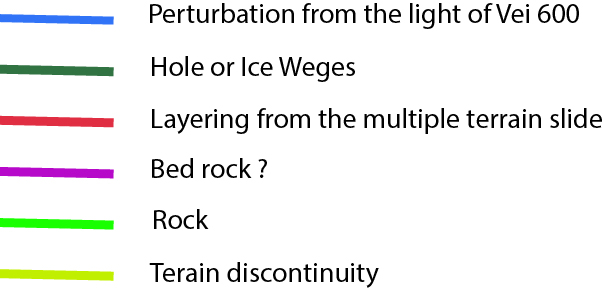
\includegraphics[width=0.5\linewidth]{Images/00_Results/Legend.jpg}
    \caption{Legend for the interpretation of the figure }
    \label{fig:legend}
\end{figure}


\subsection{Test survey}

For the test survey to test the equipment, we went walking in the streets of Longyearbyen and found a very characteristic echo from pipes under the road.

\begin{figure}[H]
    \centering
    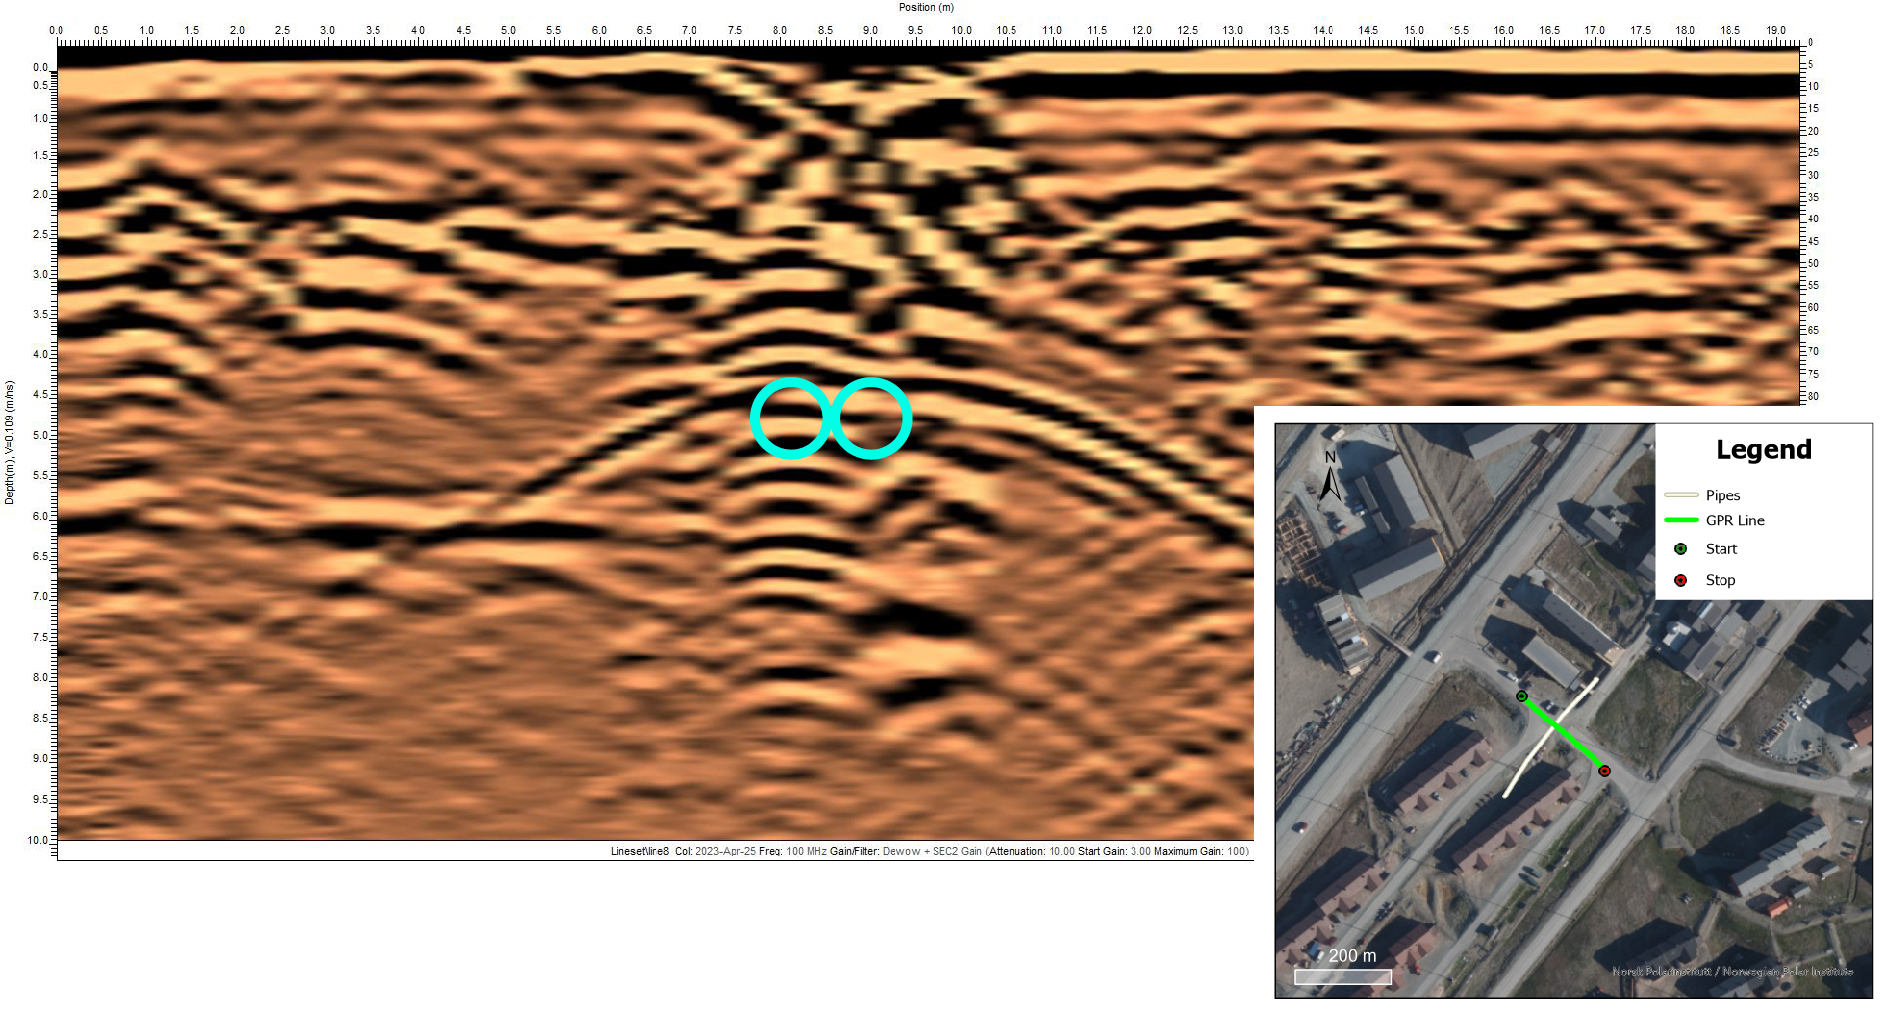
\includegraphics[width=\linewidth]{Images/00_Results/Test_line_edited.jpg}
    \caption{Test Line}
    \label{fig:testLine}
\end{figure}

The figure \ref{fig:testLine}, shows a lot of small hyperbola around the position of the pipe which is very characteristics of a single buried object. We also see some change in the upper layer due to the different materials used for the road surface.


\subsection{Main Survey}

\begin{figure}[H]
    \centering
    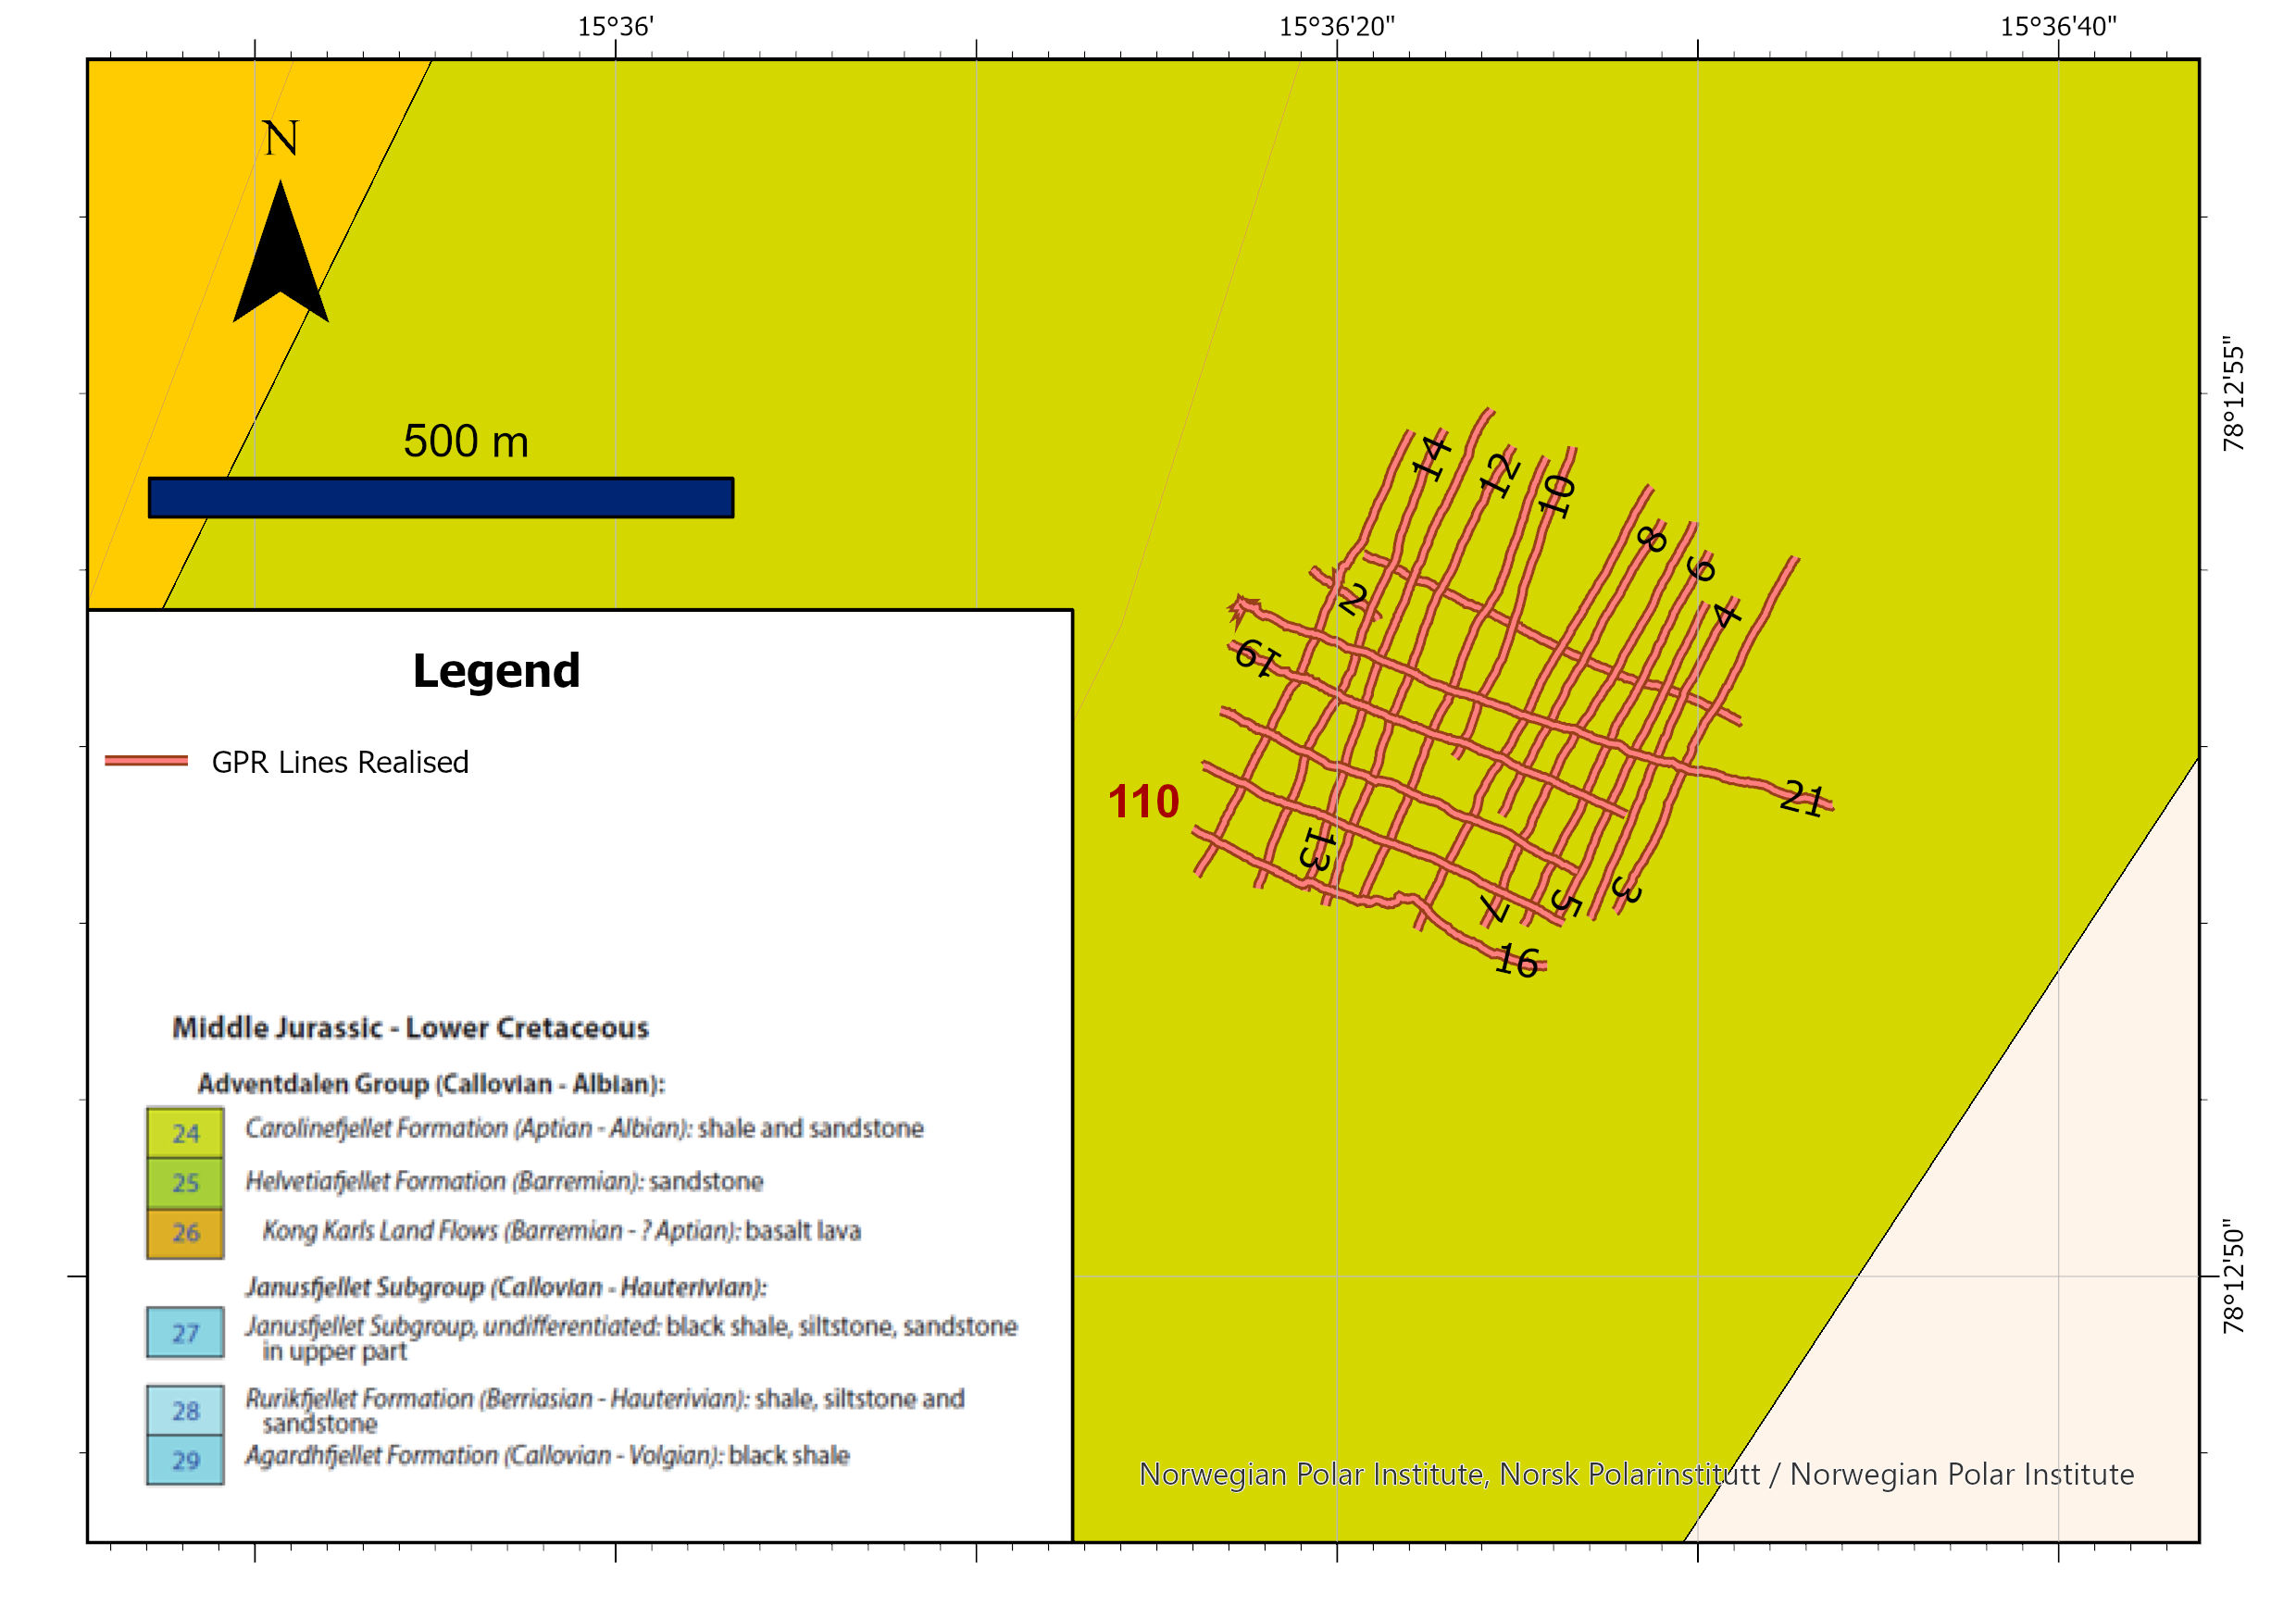
\includegraphics[width=\linewidth]{Images/00_Results/GPR LIne.jpg}
    \caption{Location of the different lines realised during the survey and the line number.}
    \label{fig:LocGPRLines}
\end{figure}

\paragraph{Results from the lines parallel to the slope} First we will present the lines realised parallel to the slope because they allow to understand some of the limitations of the GPR and the ground. During that part, when start the line 2 and 20, the fiber optic of the receiver had some connection issue and we restarted the line and didn't process it (because no data were available but only noise).

On all the lines we easily see the layering of the upper sedimentary part of the subsurface. This layering is most likely linked to the different land slides and avalanche deposits in this run out area. This layering might also be generated by some kind of interference with the pulk even if this second hypothesis is very unlikely because of the irregularity of the layering.

On the line 1 presented on figure \ref{fig:line1}, we might be able to see the bed rock (pink annotation). It's with the line 19 (figure \ref{fig:line19}) the two figures where we could see an underground layer which could correspond to the base rock. This hypothesis must be confirmed with some data providing the depth of the base rock at this position (borehole, geological archives...) and I didn't manage to find such a documentation. So according to this data the bed rock might be at a depth around 20m.

 
Unfortunately, it was the only good hyperbola to compute the velocity underground and so we get a velocity of $0.235m/ns$ which is quite high according to the velocity we could expect for permafrost area \cite{GPRAnalysis}.

Finally, we have some structure which are quite complicated to understand. My better guess is that structure could be some ice wedges as we captured in Adventdalen during the semester \cite{UNIS211-GPRReport}.

\begin{figure} [p]
    \centering
    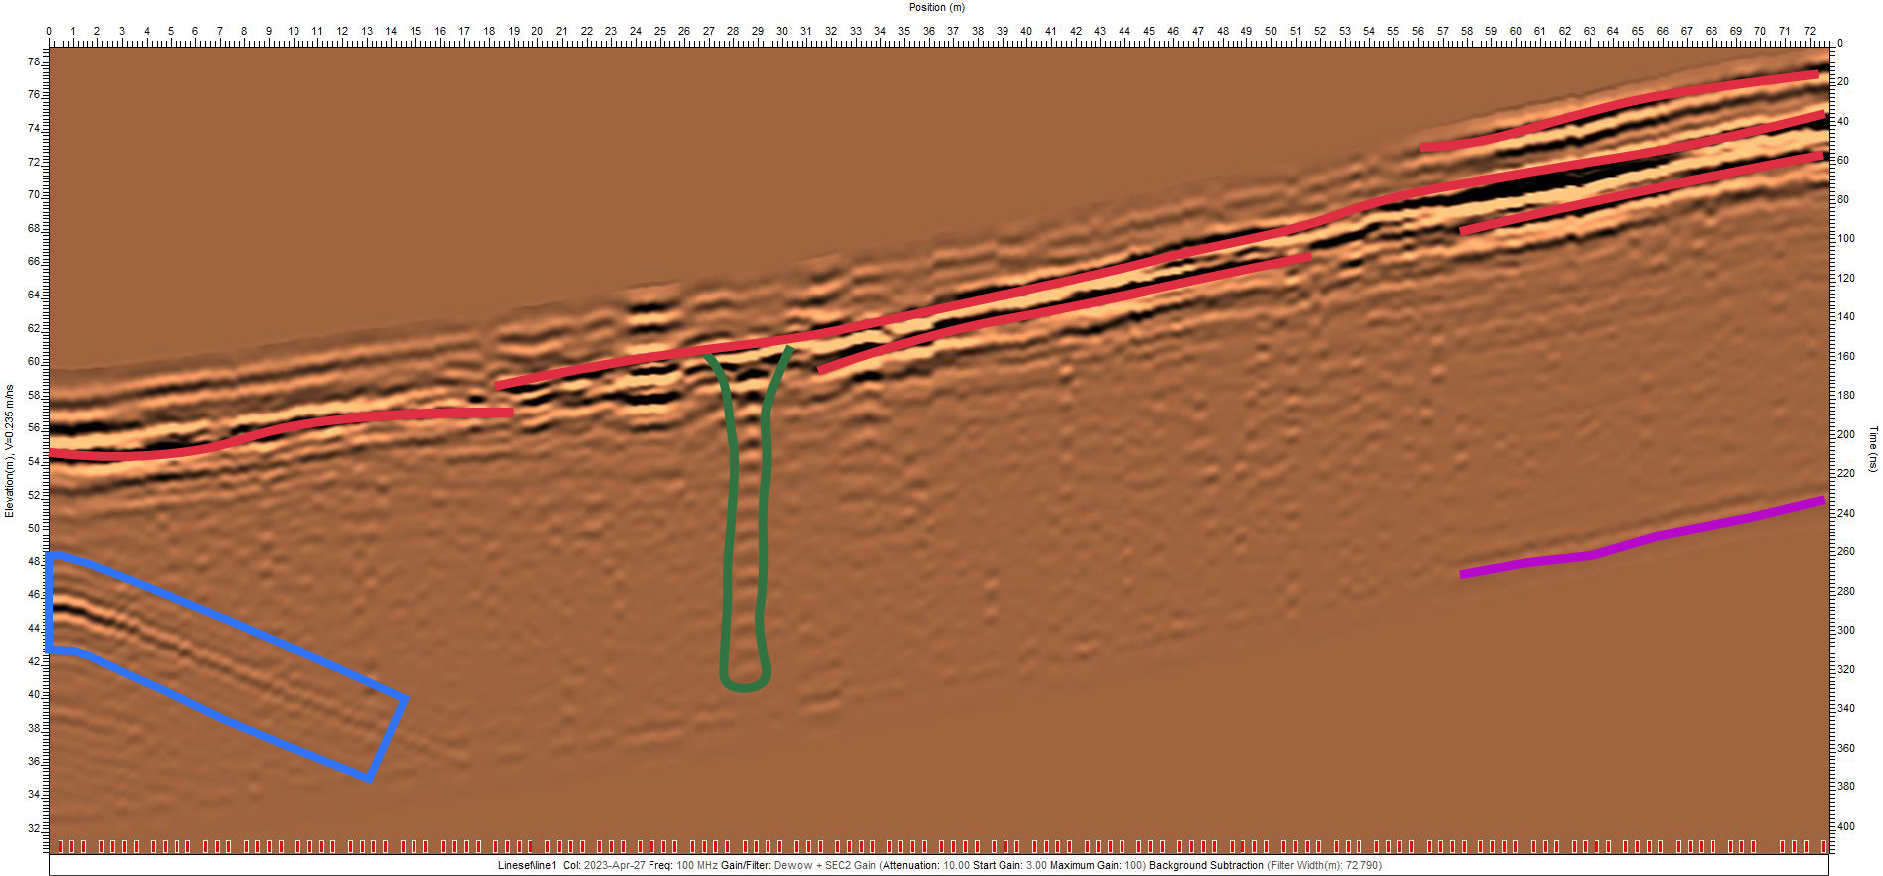
\includegraphics[width=\linewidth]{Images/00_Results/line1_edited.jpg}
    \caption{Line 1 with interpretations, legend on figure \ref{fig:legend}}
    \label{fig:line1}
\end{figure}

\begin{figure}[p]
    \centering
    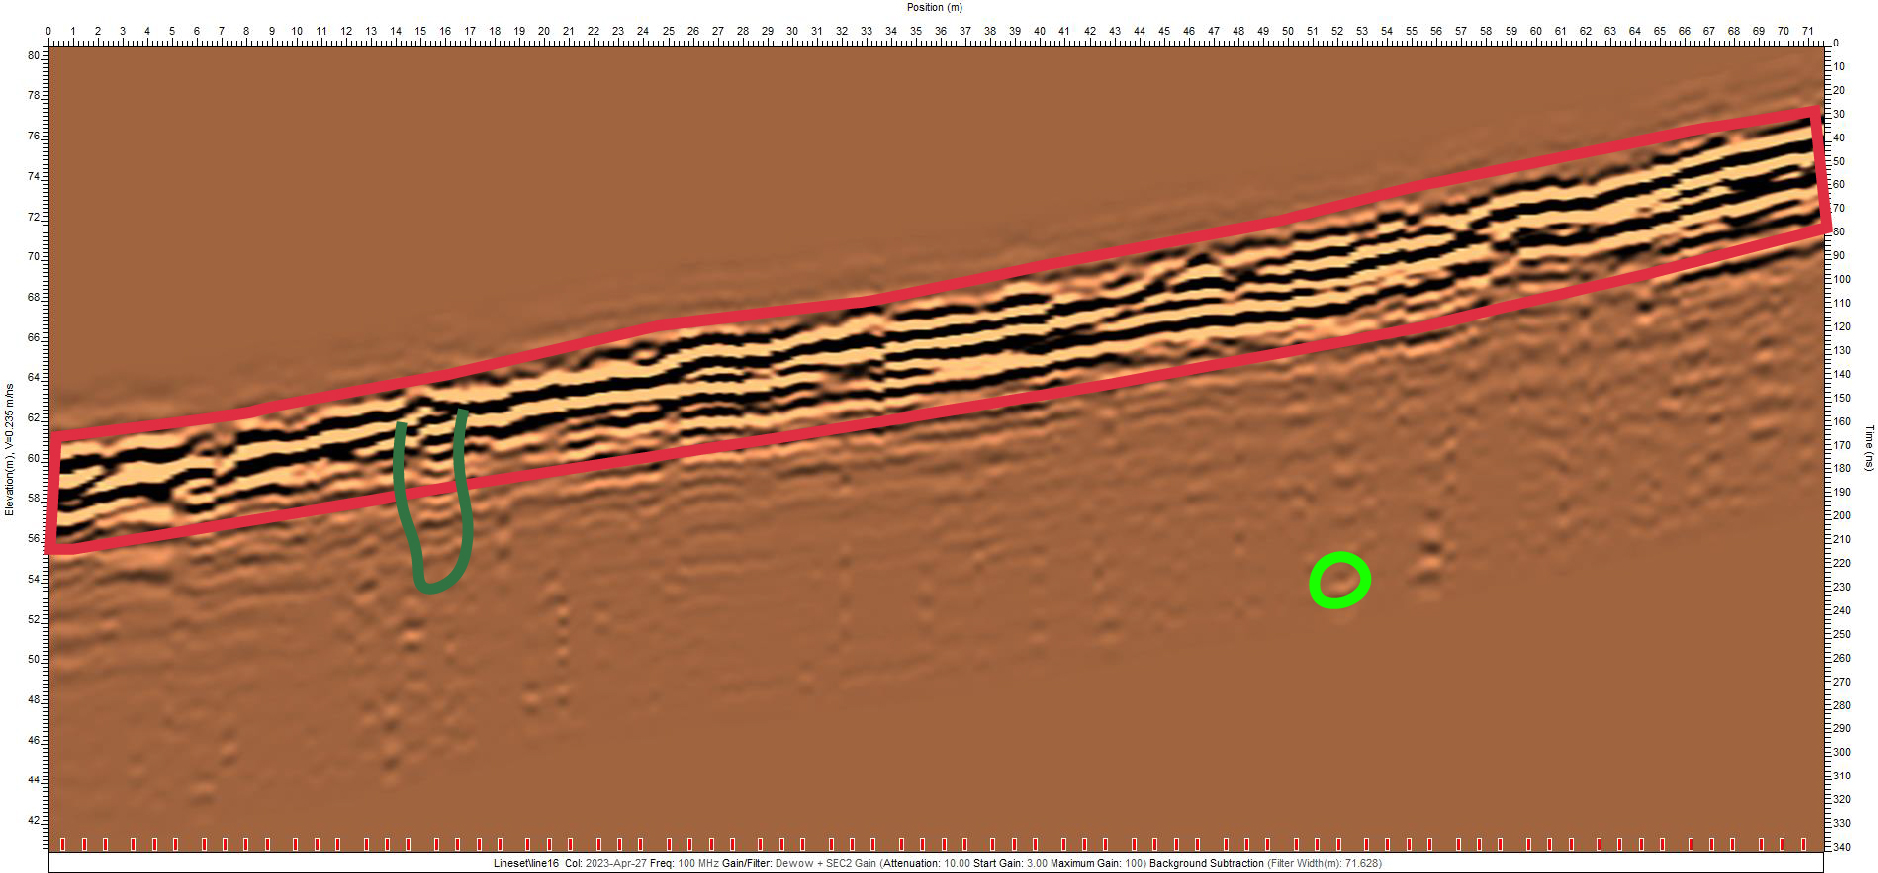
\includegraphics[width=\linewidth]{Images/00_Results/line16_edited.jpg}
    \caption{Line 16 with interpretations, legend on figure \ref{fig:legend}}
    \label{fig:line16}
\end{figure}

\begin{figure}[p]
    \centering
    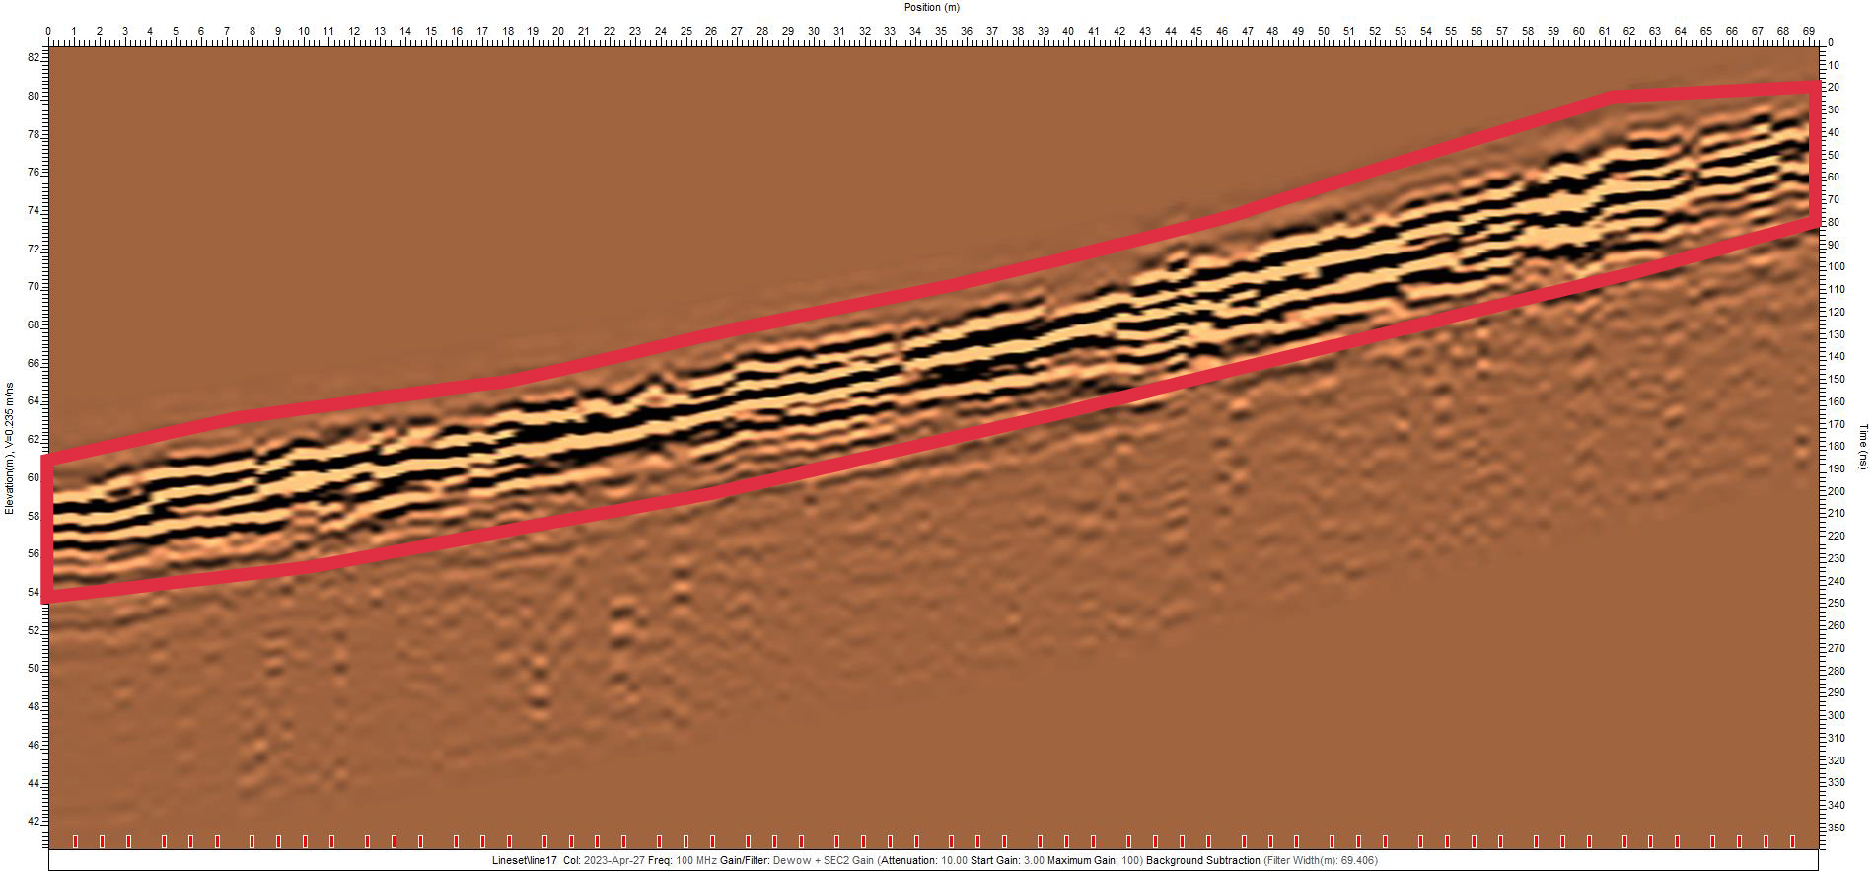
\includegraphics[width=\linewidth]{Images/00_Results/line17_edited.jpg}
    \caption{Line 17 with interpretations, legend on  figure \ref{fig:legend}}
    \label{fig:line17}
\end{figure}

\begin{figure}[p]
    \centering
    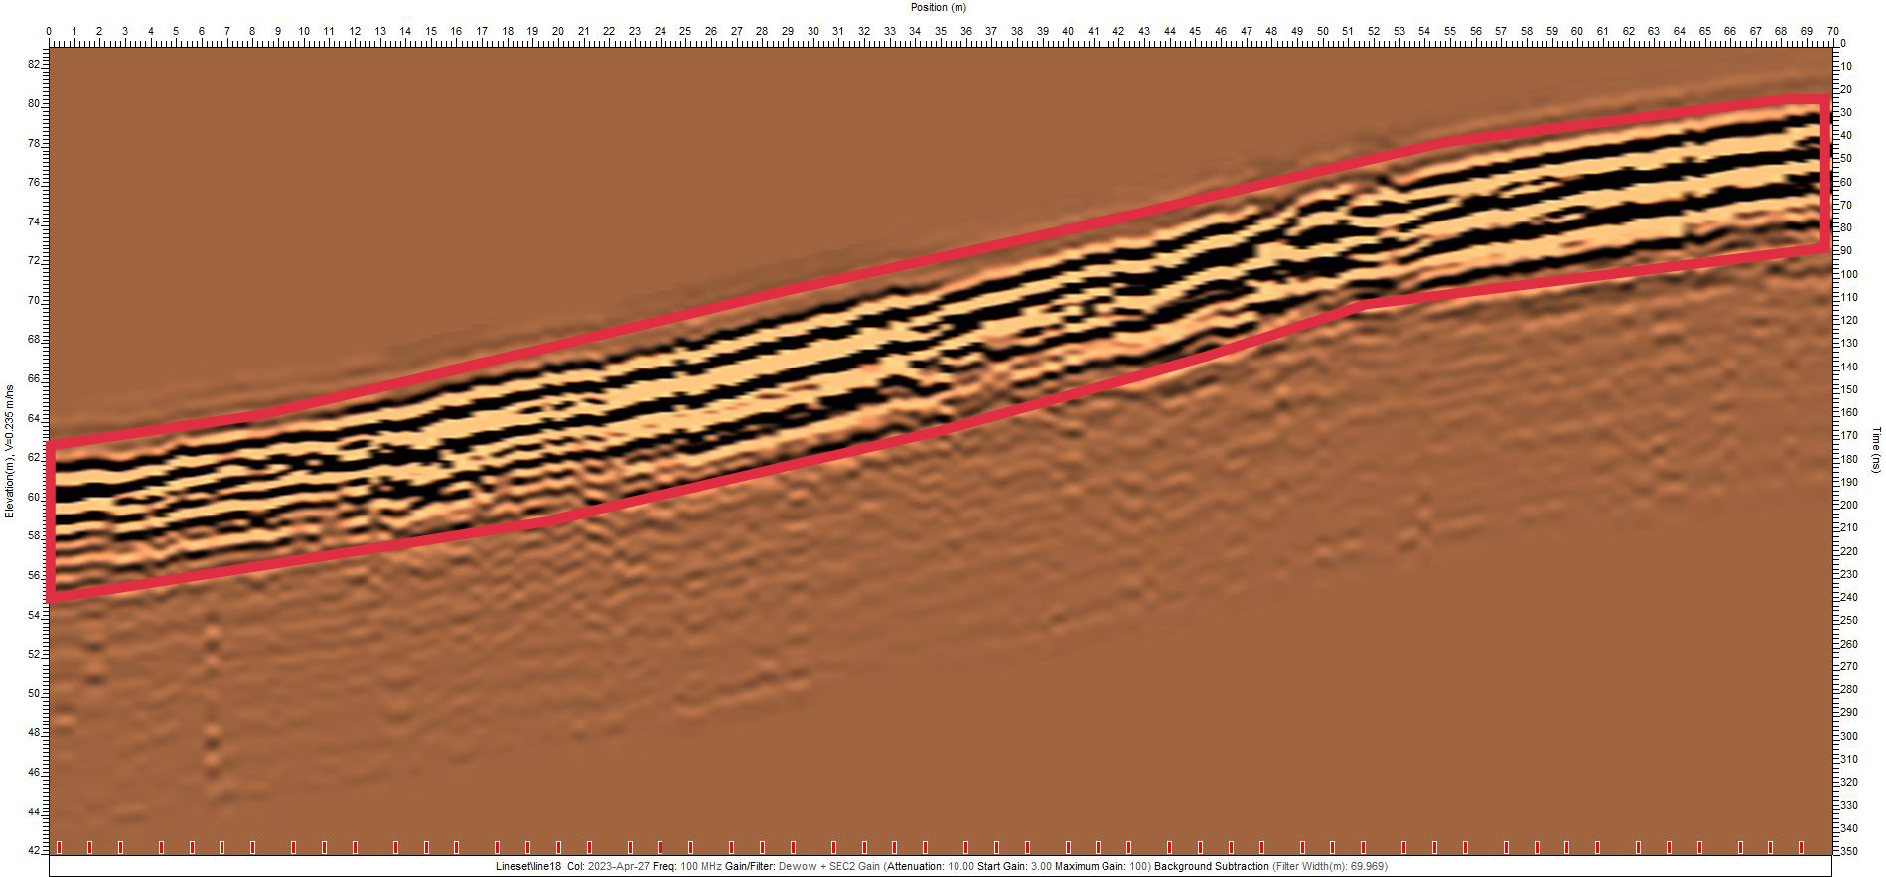
\includegraphics[width=\linewidth]{Images/00_Results/line18_edited.jpg}
    \caption{Line 18 with interpretations, legend on figure \ref{fig:legend}}
    \label{fig:line18}
\end{figure}

\begin{figure}[p]
    \centering
    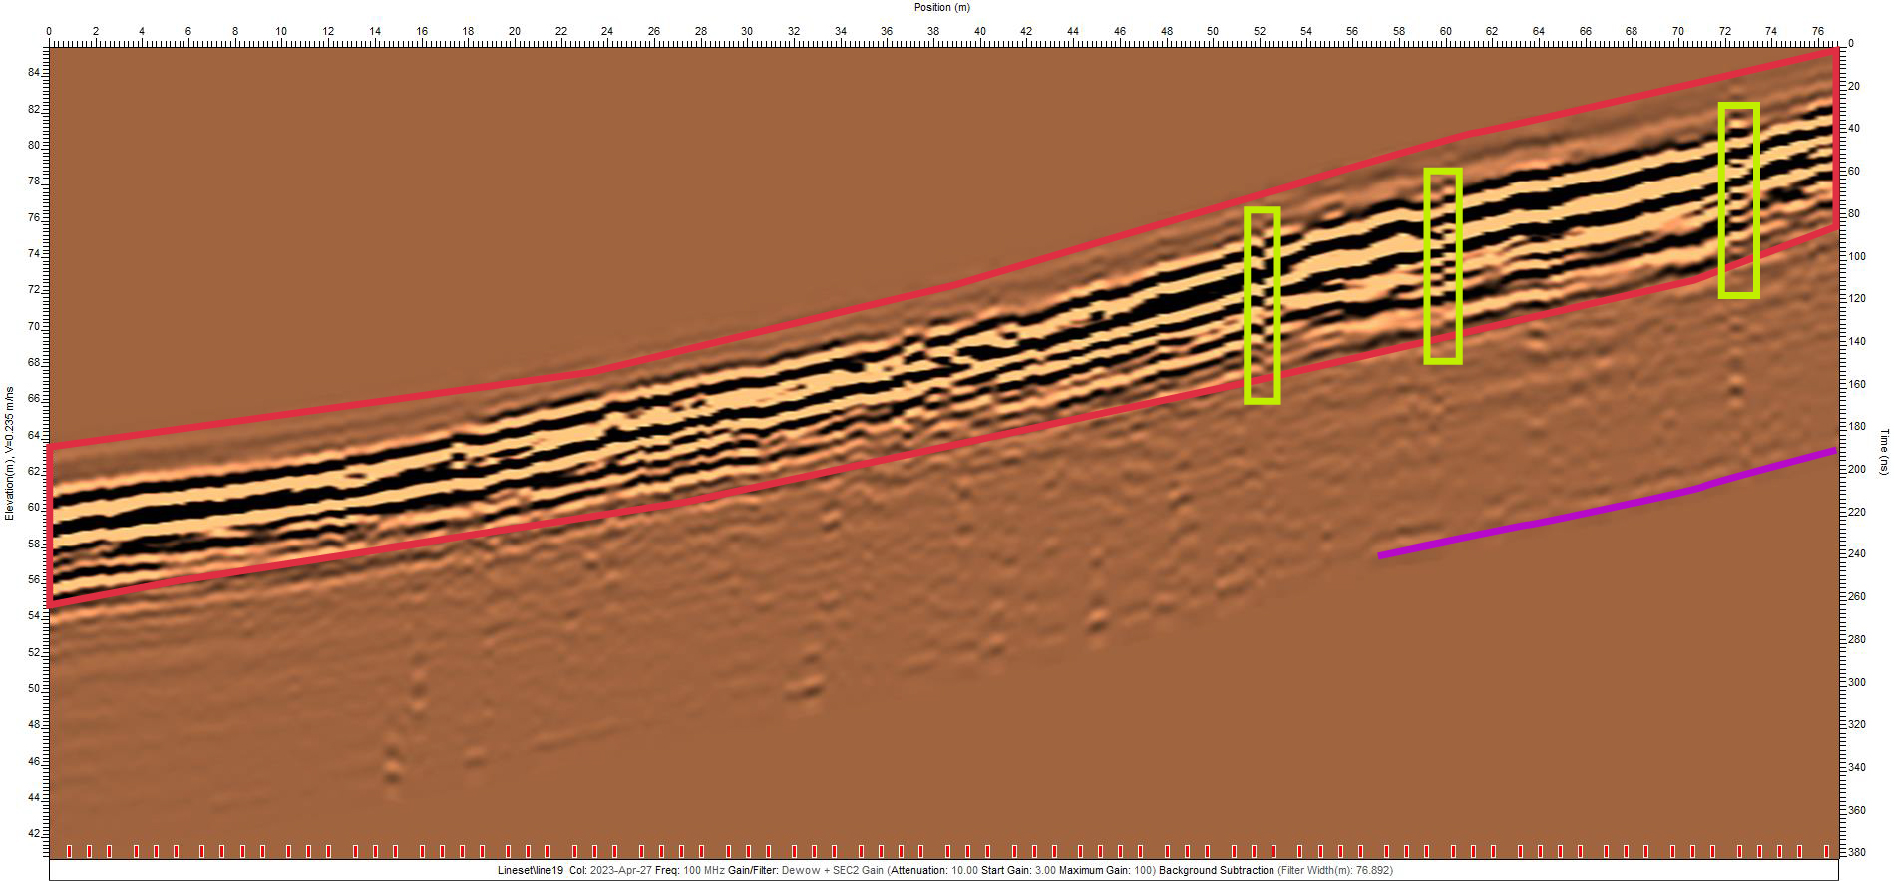
\includegraphics[width=\linewidth]{Images/00_Results/line19_edited.jpg}
    \caption{Line 19 with interpretations, legend on figure \ref{fig:legend}}
    \label{fig:line19}
\end{figure}

\begin{figure}[p]
    \centering
    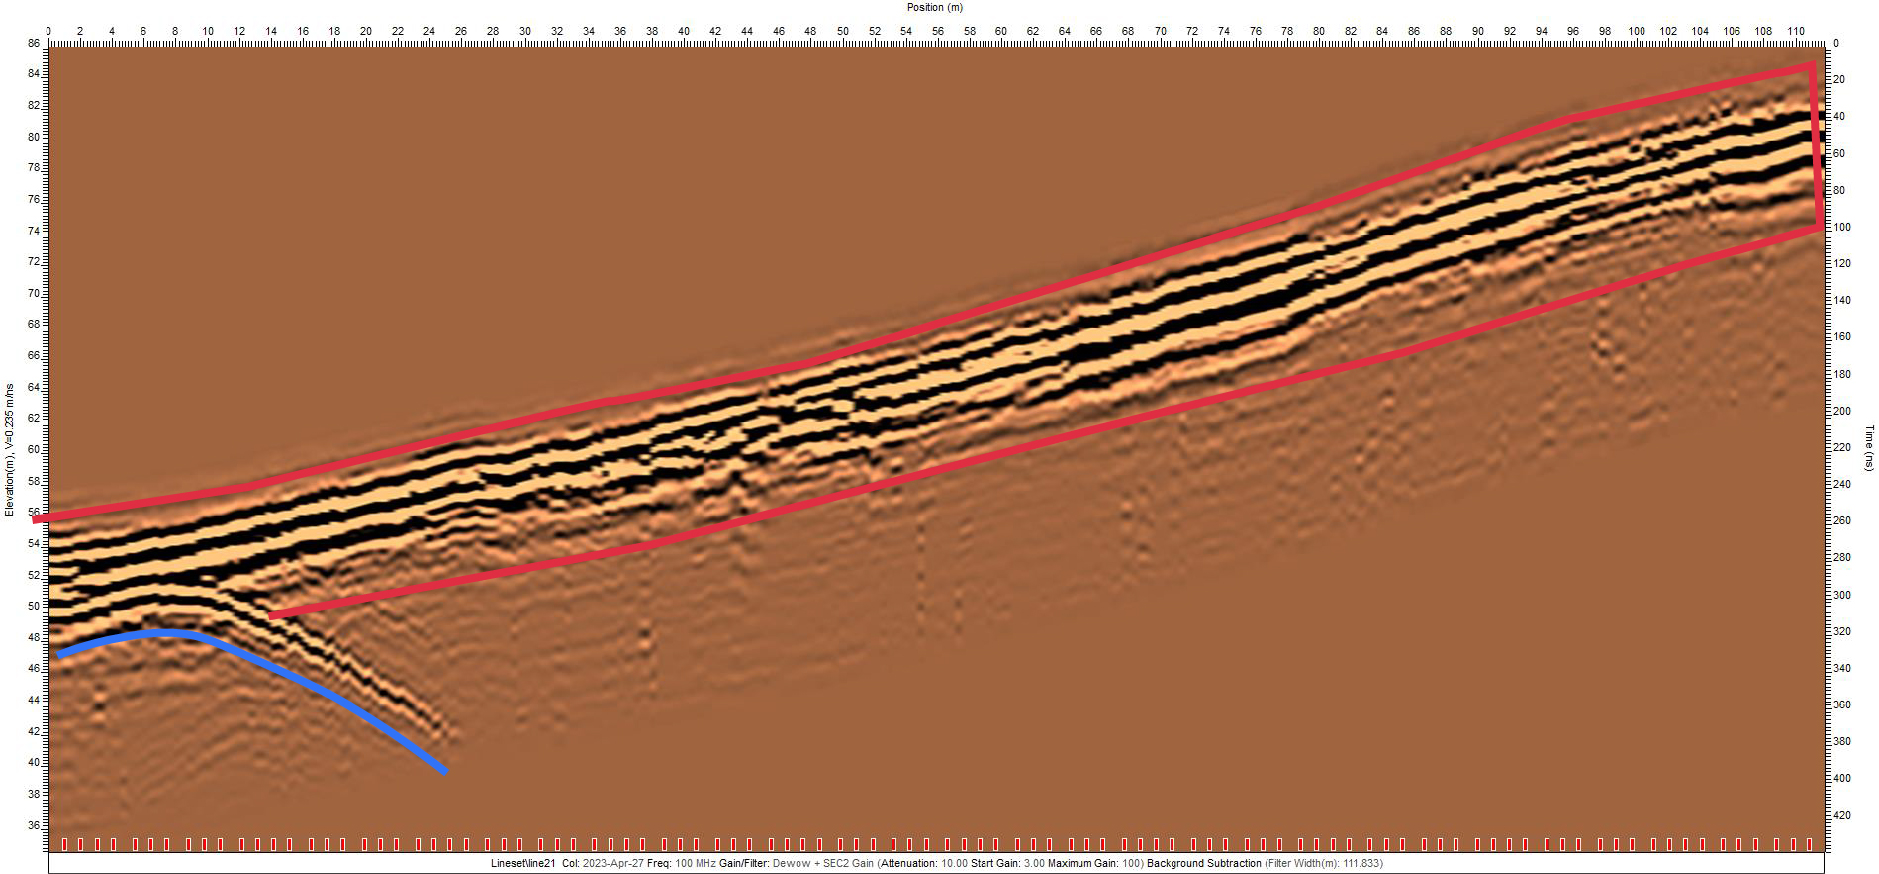
\includegraphics[width=\linewidth]{Images/00_Results/line21_edited.jpg}
    \caption{Line 21 with interpretations, legend on figure \ref{fig:legend}}
    \label{fig:line21}
\end{figure}


\newpage
\paragraph{Results from the lines perpendicular to the slope} On the horizontal lines, we see mostly only the layering on the upper part as well as sometimes few structures which might be some ice wedges. 

On lines 6 and 9 (figure \ref{fig:line6} and \ref{fig:line9}), there is a structure which is much more detailed than the rest of the lines. My knowledge and research didn't allow me to understand which is this structure and thus we have to organise additional researches to figure out.

\foreach \x in {3,4,5,6,7,8,9,10,11,12,13,14,15} {
    \begin{figure}
        \centering
        \includegraphics[width=\linewidth]{Images/00_Results/line\x_edited.jpg}
        \caption{Line \x\ with interpretations, legend on figure \ref{fig:legend}}
        \label{fig:line\x}
    \end{figure}
}
\newpage
\paragraph{Spacial representation} As we do a grid, we are able to try to represent the survey in 3D environment. For that, we just export the data from Ekko Project as a point cloud and import it in Cloud Compare in order to display the survey in 3D.

This technique is unfortunately not detailed enough to do any correct interpretations.

\begin{figure}[H]
    \centering
    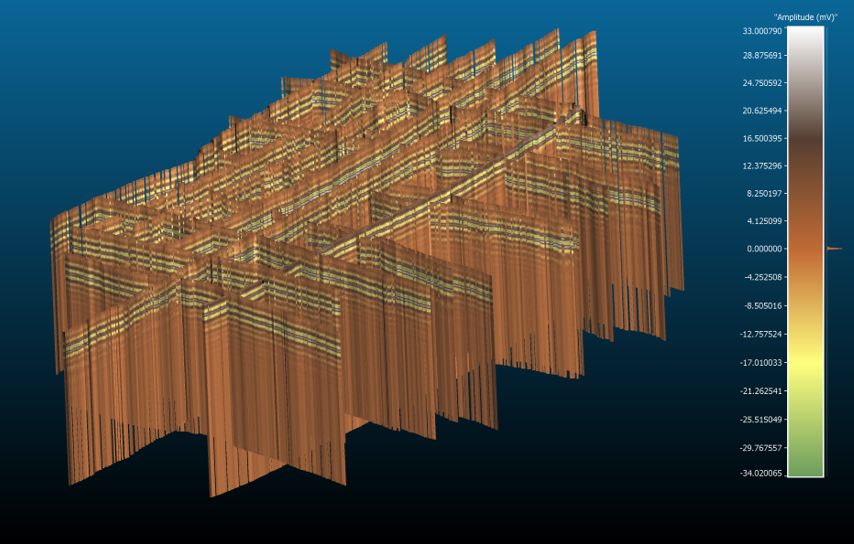
\includegraphics[width=\linewidth]{Images/00_Results/3DCloudPoint.png}
    \caption{3D representation of the survey}
    \label{fig:3D}
\end{figure}

